\documentclass{beamer}

\usepackage[utf8]{inputenc}
\usepackage{hyperref}

\usetheme{Berkeley}
\beamertemplatenavigationsymbolsempty
\setbeamertemplate{headline}{}
 
\title{Import FoodChain-Lab Workflow}
\date{}
 
\begin{document}
\maketitle
 
\section{1}
\begin{frame}
	\begin{center}
  		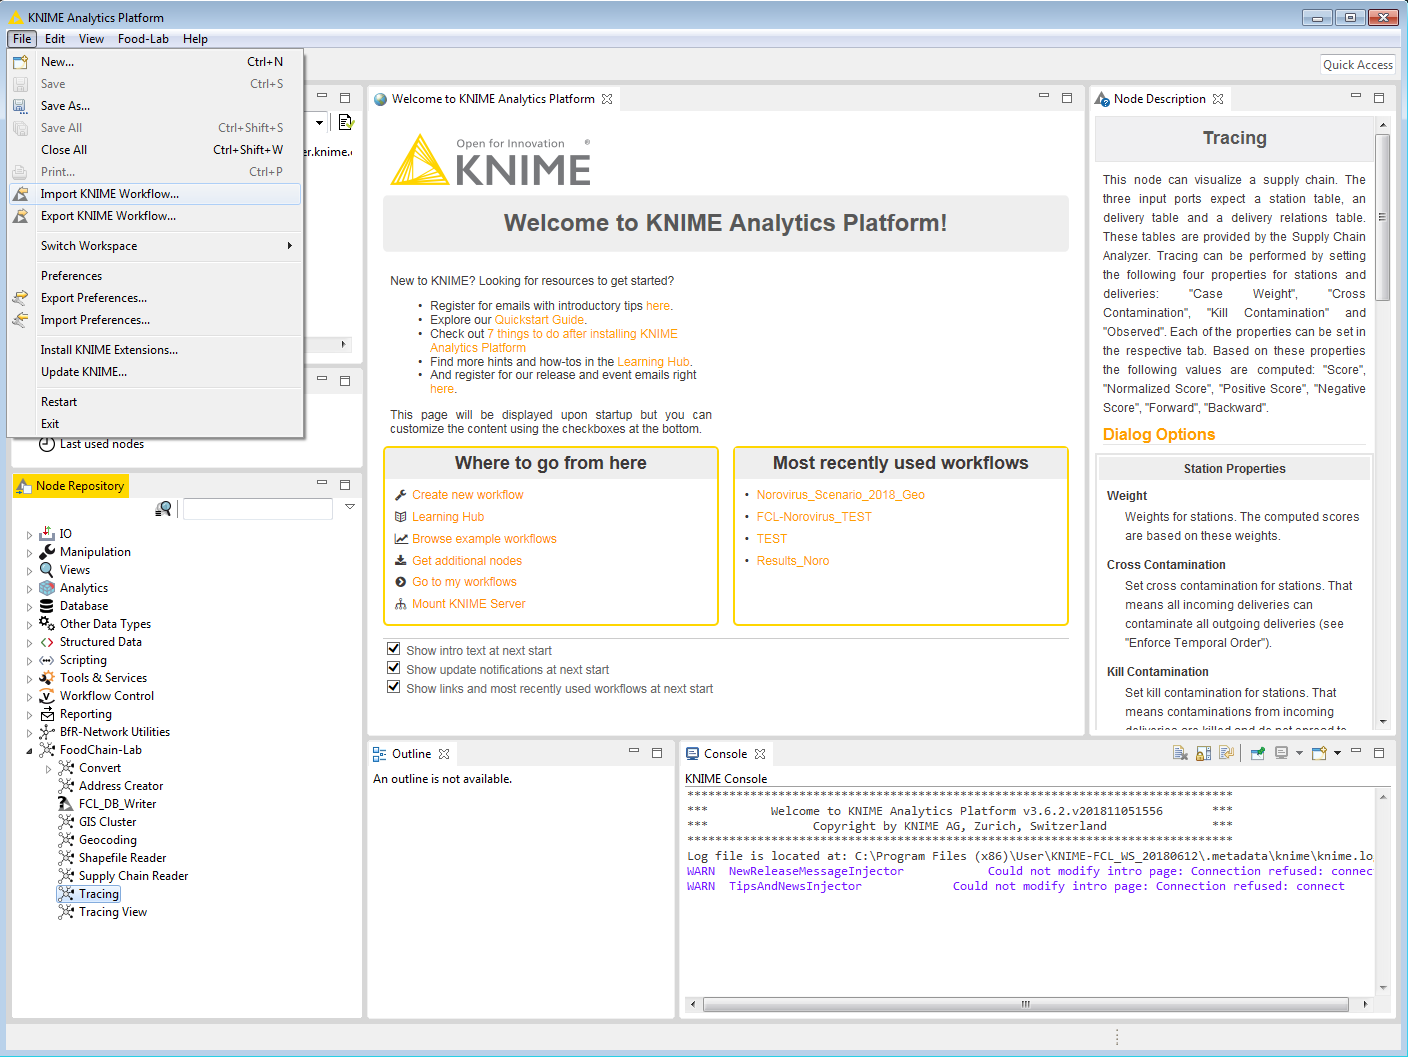
\includegraphics[height=0.6\textheight]{1.png}
	\end{center}
	\begin{itemize}
		\item Klicken Sie im \textbf{KNIME Explorer} mit einem Rechtsklick auf \textbf{LOCAL} und wählen Sie \textbf{Import KNIME Workflow} aus.
	\end{itemize}
\end{frame}

\section{2}
\begin{frame}
	\begin{center}
  		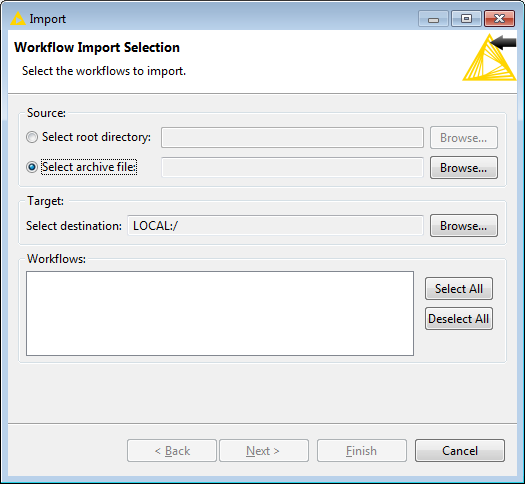
\includegraphics[height=0.6\textheight]{2.png}
	\end{center}
	\begin{itemize}
		\item Im nun erscheinenden Import-Dialog klicken Sie bitte \textbf{Select archive file} an und klicken rechts auf \textbf{Browse}.
	\end{itemize}
\end{frame}

\section{3}
\begin{frame}
	\begin{center}
  		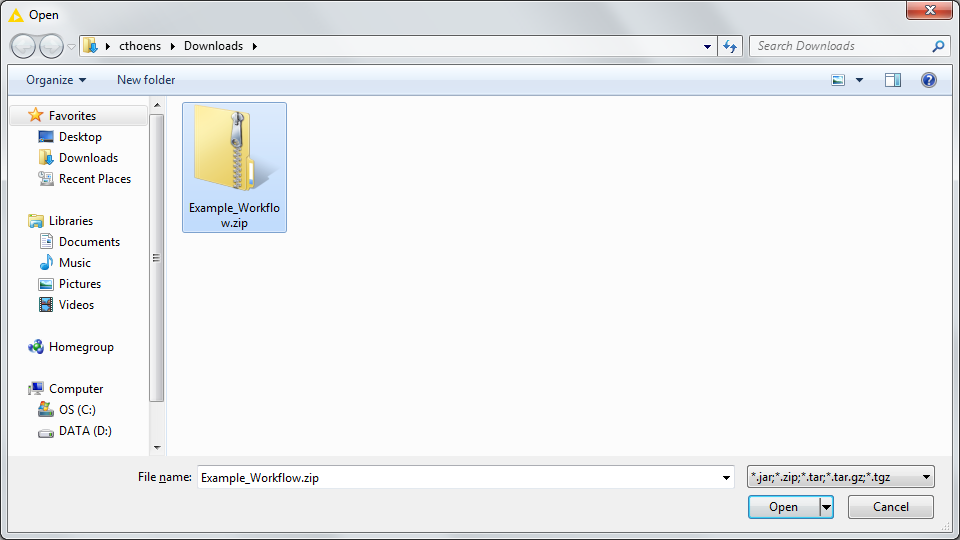
\includegraphics[height=0.6\textheight]{3.png}
	\end{center}
	\begin{itemize}
		\item Wählen Sie einen gezippten Workflow-Ordner aus, den Sie auf Ihrem Dateisystem gespeichert haben. Klicken Sie auf \textbf{Open}.
		\item Beispiel Workflow: \url{https://github.com/SiLeBAT/BfROpenLabResources/raw/master/GitHubPages/workflows/Example_Workflow.zip}
	\end{itemize}
\end{frame}

\section{4}
\begin{frame}
	\begin{center}
  		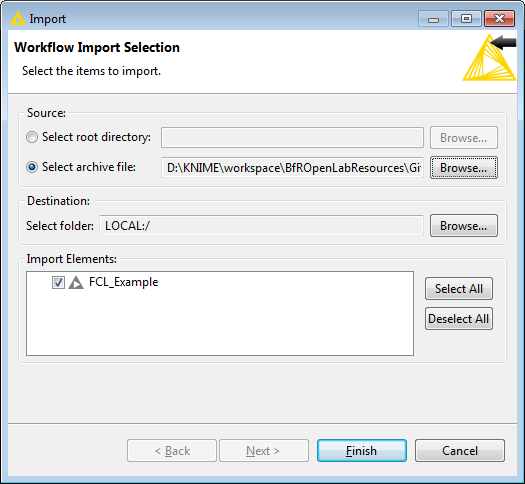
\includegraphics[height=0.6\textheight]{4.png}
	\end{center}
	\begin{itemize}
		\item Der gewählte Workflow sollte nun im Import-Dialog zu sehen sein. Klicken Sie auf \textbf{Finish}.
	\end{itemize}
\end{frame}

\section{5}
\begin{frame}
	\begin{center}
  		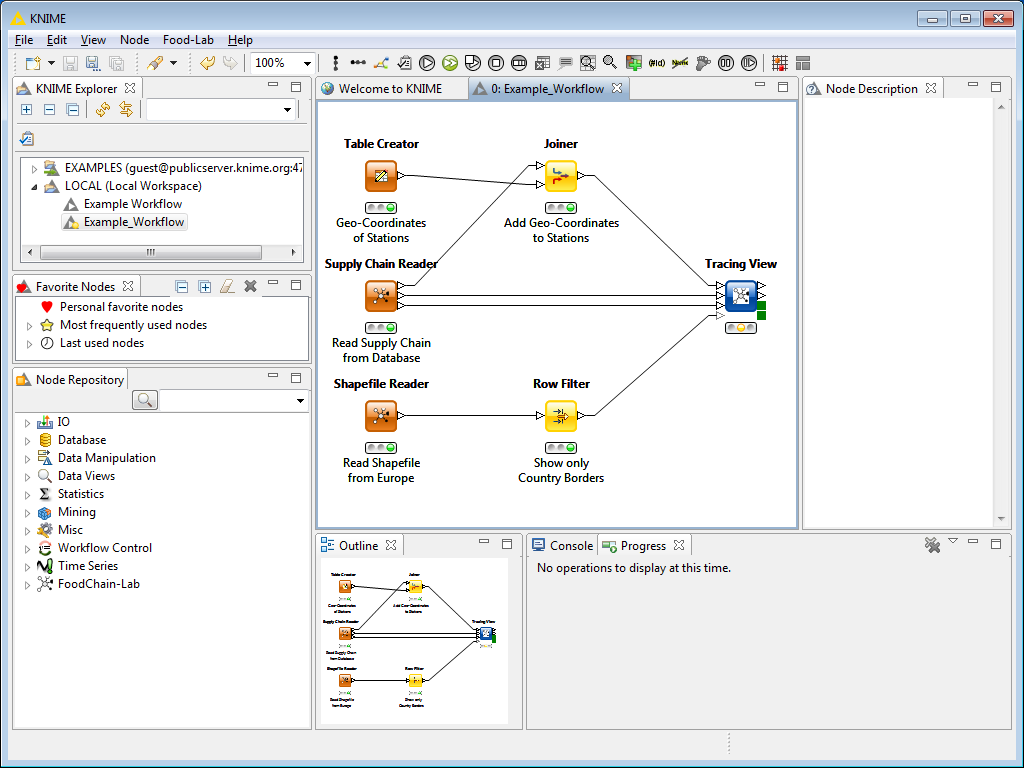
\includegraphics[height=0.6\textheight]{5.png}
	\end{center}
	\begin{itemize}
		\item Klicken Sie auf den kleinen Pfeil neben \textbf{LOCAL} im \textbf{KNIME Explorer}, um alle vorhandenen Workflows anzuzeigen. Zum Öffnen eines Workflows klicken Sie mit einem Doppelklick darauf. Er öffnet sich anschließend im großen zentralen Editor-Fenster.
	\end{itemize}
\end{frame}

\end{document}